\chapter{Parte teórica y desarrollo del código}
El paquete \texttt{solaR2} toma como marco teórico el libro de Oscar Perpiñán, tutor de este trabajo, Energía Solar Fotovoltaica \cite{Perpinan2023} para cada una de las operaciones de cálculo que realizan cada una de las funciones.
En la figura \ref{fig:orgbd45819}, se muestra un diagrama que resume los pasos que se siguen a la hora de calcular la producción de sistemas fotovoltaicos.
\begin{figure}[p]
\centering
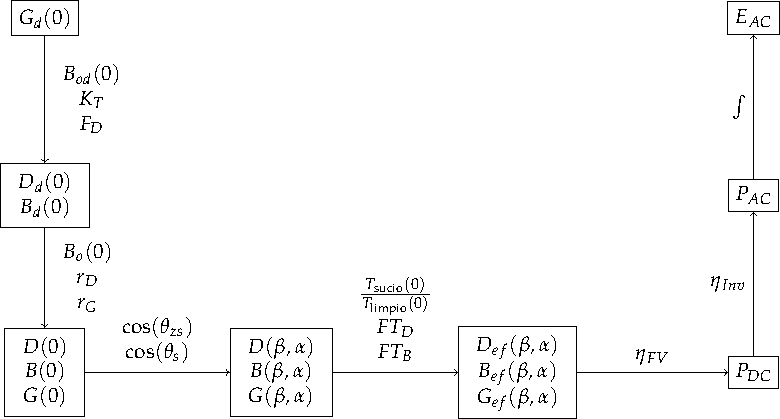
\includegraphics[keepaspectratio,width=0.9\textwidth,height=0.5\textheight]{figuras/ProcedimientoCalculoRadiacionInclinada.pdf}
\caption{\label{fig:orgbd45819}Procedimiento de cálculo}
\end{figure}
Estos pasos son:
\begin{enumerate}
\item Obtener la irradiación global diaria en el plano horizontal
\item A partir de la irradiación global, obtener las componentes de difusa y directa.
\item Se trasladan estos valores de irradición a valores de irradiancia.
\item Con estos valores se pueden obtener los valores correspondientes en el plano del generador
\begin{enumerate}
\item Sin los efectos de la suciedad de los modulos y las sombras que se generan unos con otros.
\item Con estos efectos
\end{enumerate}
\item Integrando estos valores se pueden obtener las estimaciones irradiación diaria difusa, directa y global
\item El generador fotovoltaico produce una potencia en corriente continua dependiente del rendimiento del mismo..
\item Se transforma en potencia en corriente alterna mediante un inversor que tiene una eficiencia asociada.
\item Integrando esta potencia se puede obtener la energía que produce el generador en un tiempo determinado.
\end{enumerate}
En la figura \ref{fig:orge3c8a79}, se muestra el proceso de cálculo que sigue el paquete a la hora de obtener la estimación de la producción del sistema fotovoltaico.
\begin{figure}[p]
\centering
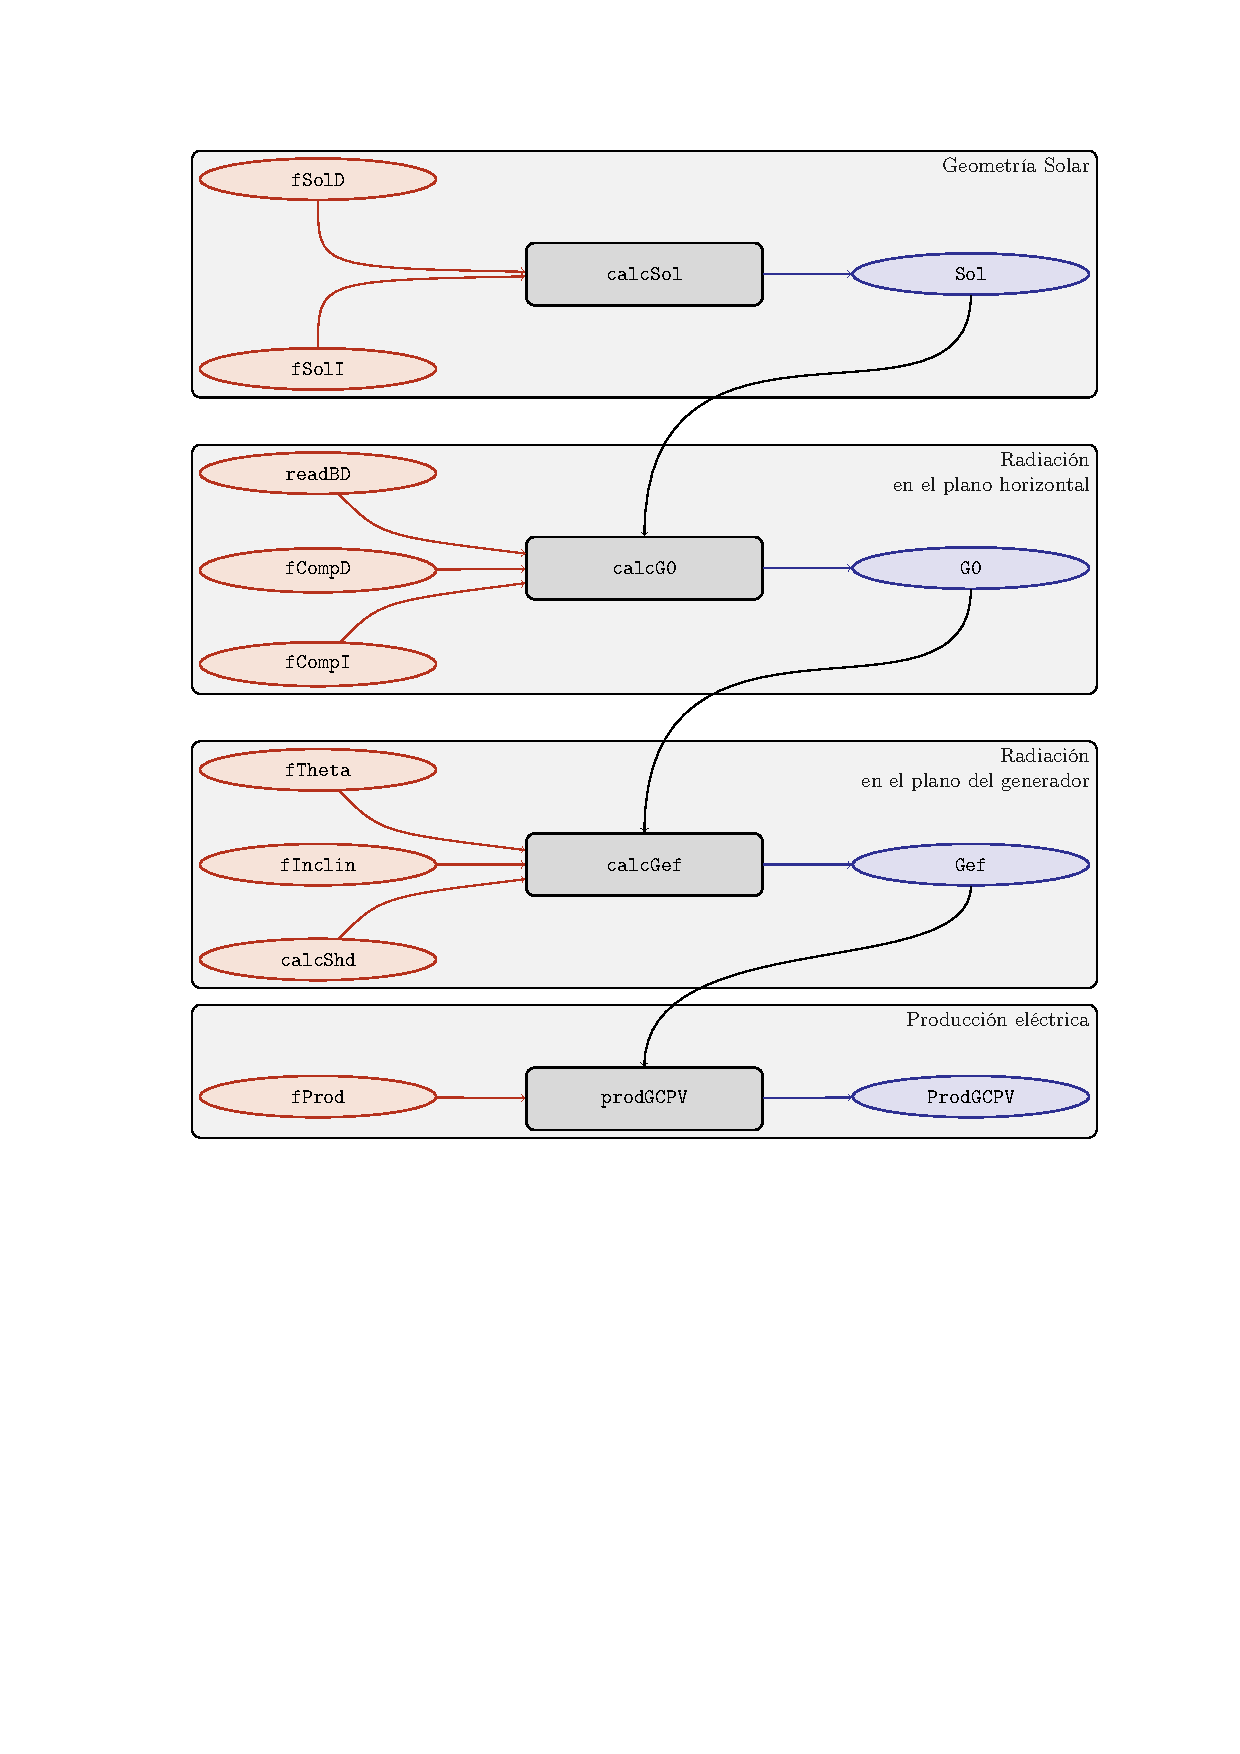
\includegraphics[keepaspectratio,width=0.9\textwidth,height=0.5\textheight]{figuras/procedure.pdf}
\caption{\label{fig:orge3c8a79}Proceso de cálculo de las funciones de \texttt{solaR2}}
\end{figure}
A la hora de estimar la producción, el programa sigue los siguientes procesos:
\begin{enumerate}
\item Se calcula la geometría que definen la posición de la Tierra frente al Sol
\begin{enumerate}
\item Mediante la función fSolD, se calculan:
\begin{itemize}
\item El ángulo de declinación de la Tierra (\(\delta\)\nomenclature[delta]{\(\delta\)}{Declinación}).
\item La corrección debida a la excentricidad de la elipse de la trayectoria terrestre alrededor del sol (\(\epsilon_0\)\nomenclature[epsilon0]{\(\epsilon_0\)}{Corrección debida a la excentricidad de la elipse de la trayectoria terrestre alrededor del sol}).
\item La ecuación del tiempo (\(EoT\)\nomenclature{\(EoT\)}{Ecuación del tiempo}).
\item El ángulo del amanecer (\(\omega_s\)\nomenclature[omegas]{\(\omega_s\)}{Ángulo del amanecer}).
\end{itemize}
\item Mediante la función fSolI, se calculan:
\begin{itemize}
\item La hora solar (\(\omega\)\nomenclature[omega]{\(\omega\)}{Hora solar o tiempo solar verdadero}).
\item El momento del día en el que es de noche.
\item El ángulo cenital solar (\(\theta_{zs}\)\nomenclature[thetazs]\{\(\theta\)\textsubscript{zs}$\backslash$}\{Ángulo cenital solar\}).
\item El ángulo de altura solar (\(\gamma_s\)\nomenclature[gammas]{\(\gamma_s\)}{Altura solar}).
\item El ángulo azimutal solar (\(\psi_s\)\nomenclature[psis]{\(\psi_s\)}{Ángulo azimutal solar}).
\item La irradiancia extra-terrestre en el plano horizontal (\(B_0(0)\)\nomenclature{\(B_0(0)\)}{Irradiancia extra-atmosférica o extra-terrestre en el plano horizontal}).
\end{itemize}
\item El resultado de ambas funciones se juntan en un solo objeto de clase \texttt{Sol}
\end{enumerate}
\item Se calcula la radiación en el plano horizontal
\begin{enumerate}
\item 
\end{enumerate}
\end{enumerate}
